



\subsection{Related Work}
\begin{figure}[t]
  \centering
  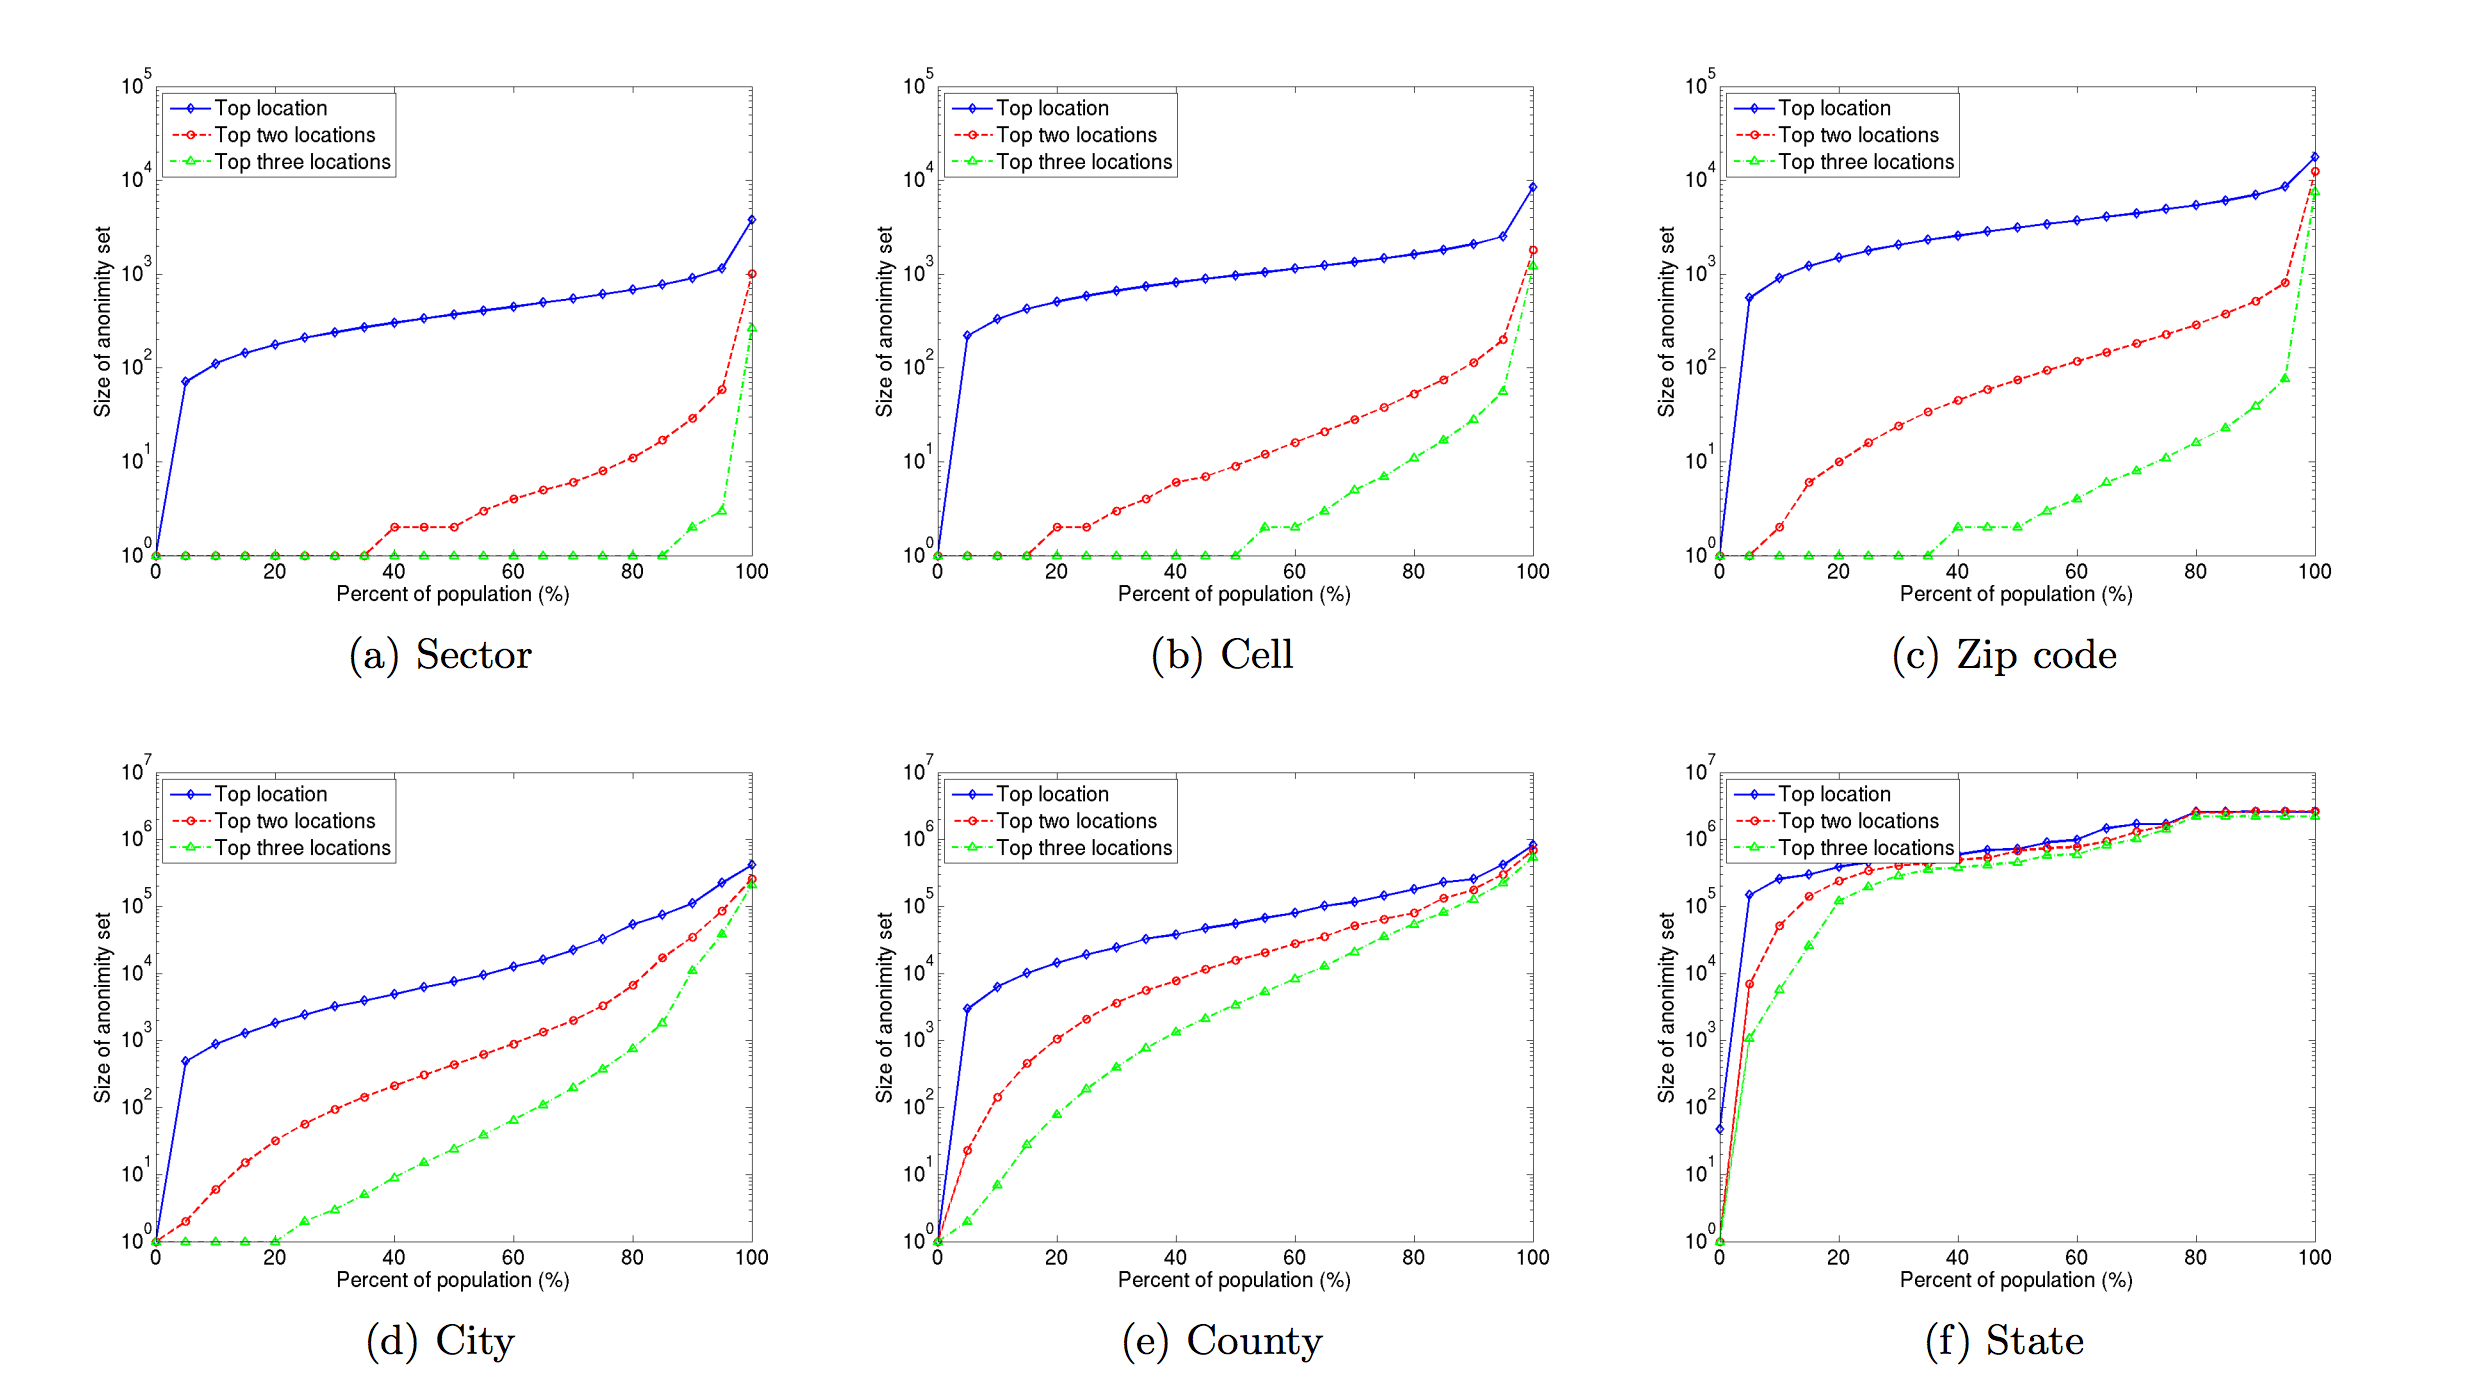
\includegraphics[width=\linewidth]{fig/zang_bolot.png}
  \caption{Figure from~\ref{Zang:2011hk} depicting the size of anonymity sets for top $n$ most visited location of users.
           Locations are varied in granularity, from cell sectors to US states.}
  \label{fig:zang_bolot}
\end{figure}

Location data for individuals is highly unique and thus difficult to anonymize.
The first large-scale study of the $k$-anonymity of location data was appropriately titled ``Anonymization of Location Data Does Not Work"~\ref{Zang:2011hk}.
The paper used data from cell phone call detail records (or CDR, see~\chap{sec:background}) for 25 million United States users over a 3 month period.
The authors represents each user as simply their top $n$ most visited locations, varying $n$ from 1 to 3.
Additionally, the authors varied the granularity of the locations, with the smallest as cell sector and the largest as state.
Remarkably, using 3 locations at a cell level made half of all users completely unique, and 3 locations a sector level made 85\% of all users unique.
A figure detailing this result and results for other granularities and values of $n$ is depicted in~\fig{fig:zang_bolot}.
The authors went on to analyze the impact of geography (comparing different states and cities), mobility (distances between top locations), and social networks on anonymity.


The Montjoye nature report


\subsection{Completed Work}
I have investigated the anonymity of location data for users

Although prior work showed location to be highly \emph{unique} and thus posibly \emph{vulnerable} to de-anonymization, no data was actually de-anonymized in practice.
Indeed, just because a data source is highly unique does not mean it can be de-anonymized.
For example, much of cryptography relies on creating highly unique but unpredictable sequences of numbers.
To put it more concretely, imagine that each individual had a die with 1000 sides, and each side represented a location.
If, quite hypothetically, humans decided where to go next by rolling this die, their movements would look very unique.
However, since the movements are random and unpredictable, my movements from different time periods will be indistinguishable from those of a different individual.

TODO: put some math here?

Another possibile break in the argument that uniqueness implies vulnerability is the important factor of sampling.
The datasets dealt with here (phone records, social media posts) are all \emph{actively} collected: each data point exists if and only if the user has taken an action.
Intuitively, the location data from different sampling data sources should look very different.
An individual may be more likely to make phone calls in quiet places, like the home or office, and take geotagged location photos in popular tourist destinations or restaurants.

TODO: put some math here?

In ``Linking Users Across Domains with Location Data", published at WWW in 2016, we tackled this problem, linking users across two entirely different datasets.


To conduct this work, we obtained three datasets.
This in itself was a significant challenge, as each dataset needed to contain individuals with identities linked across two different data sources.
\begin{itemize}
  \item Cell phone-Credit Card
  \item Instagram-Twitter
  \item Foursquare-Twitter
\end{itemize}



and

FindYou
